\documentclass[tikz,border=2pt]{standalone}
\usepackage{tikz}
\usetikzlibrary{positioning, shapes.geometric}
\usetikzlibrary{patterns,snakes}
\begin{document}
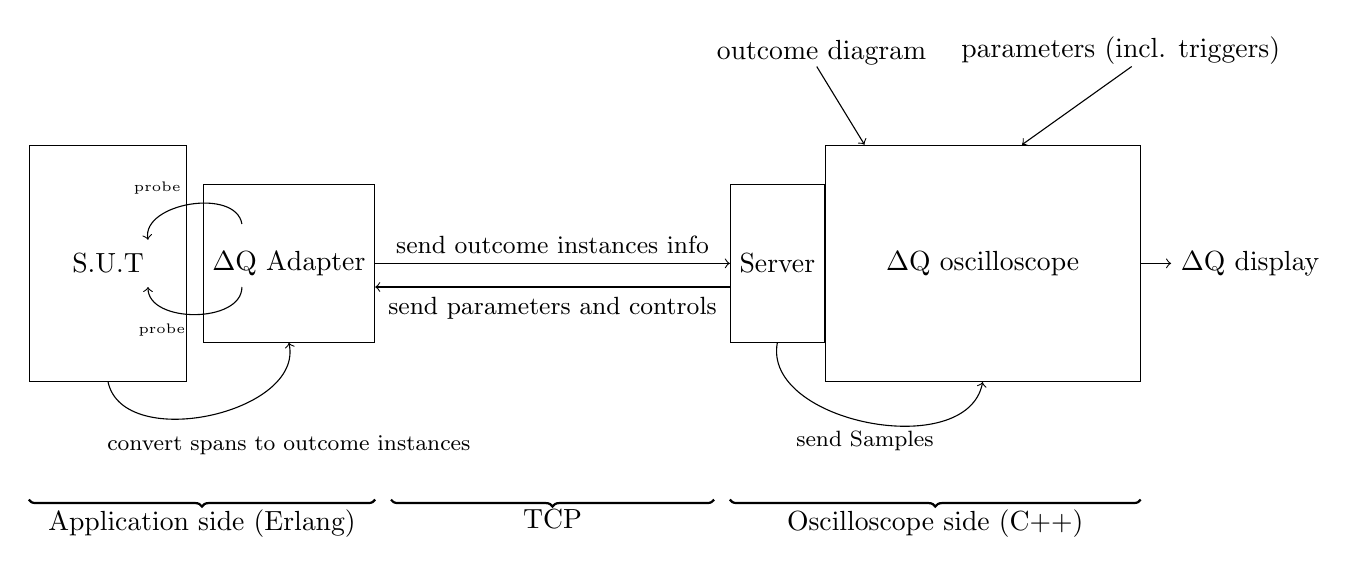
\begin{tikzpicture}

\node[rectangle,draw, minimum height = 3cm, minimum width = 2cm] (sut) at (-4, 0) {S.U.T};
\node[rectangle,draw, minimum height = 2cm, minimum width = 1cm, right of = sut, anchor = west, xshift = 0.2cm] (stub) {$\Delta$Q Adapter};

    \draw [->] (sut.south) to [bend right = 90] (stub.south) node[below=30pt] {\footnotesize convert spans to outcome instances};


    \node [rectangle, draw, minimum height = 2cm, minimum width = 1cm] (server) at (4.5, 0) {Server};

    \draw [->] (stub.east) -- (server.west) node[midway, above] {\small send outcome instances info};


    \draw [->] ([yshift=-0.3cm]server.west) -- ([yshift=-0.3cm]stub.east) node[midway, below] {\small send parameters and controls};


    \draw [->] ([yshift=0.5cm, xshift=0.5cm]stub.west) to [bend right = 90] node [above left, midway ] {\tiny probe} ([yshift=0.3cm, xshift=-0.5cm] sut.east) ;

    \draw [->] ([yshift=-0.3cm, xshift=0.5cm]stub.west) to [bend left = 90] node [below left, midway ] {\tiny probe} ([yshift=-0.3cm, xshift=-0.5cm] sut.east);

    \node [rectangle, draw, minimum height = 3cm, minimum width = 4cm, anchor = west] (osc) at(5.1, 0) {$\Delta$Q oscilloscope};

    \draw [->] (server.south) to [bend right = 90] (osc.south)  node[below left=20pt] {\footnotesize send Samples};

    \draw [->] (5, 2.5) -- ([xshift=-1.5cm]osc.north) node[pos=0.1, above] {outcome diagram};

    \draw [->] (9, 2.5) -- ([xshift=0.5cm]osc.north) node[pos=0.1, above] {parameters (incl. triggers)};

    \draw[->] (osc.east) -- (9.5, 0) node[right] {$\Delta$Q display};

    \draw [
    thick,
    decoration={
        brace,
        mirror,
        raise=3cm
    },
    decorate
] (sut.west) -- (stub.east)
    node [pos=0.5,anchor=north,yshift=-3cm] {Application side (Erlang)};


    \draw [
    thick,
    decoration={
        brace,
        mirror,
        raise=3cm
    },
    decorate
] ([xshift=0.2cm]stub.east) -- ([xshift=-0.2cm]server.west)
node [pos=0.5,anchor=north,yshift=-3cm] {TCP};


\draw [
    thick,
    decoration={
        brace,
        mirror,
        raise=3cm
    },
    decorate
] (server.west) -- (osc.east)
node [pos=0.5,anchor=north,yshift=-3cm] {Oscilloscope side (C++)};


    \end{tikzpicture}
\end{document}
